
\chapter{Oracles}
\label{chapter:oracles}

\newcommand{\leaf}{leaf bot}

This chapter refines the notion of a microprediction oracle, and infers some minimal properties. An oracle is:

\begin{quote}{Microprediction oracle definition}
An apparatus that you can reward for a frequently repeated prediction task, on an ongoing basis, with the expectation that the accuracy will be {\em eventually hard to beat} on a dollar for dollar basis. 
\end{quote}
The physical manifestation is not our immediate concern - although we imagine a formula in an Excel spreadsheet, a Python function, a callback in a web application, a programming interface, or some use of an event processing or messaging system.  

 

\section{Eventually hard to beat}

In computer science and mathematics, the term oracle is used differently. It refers to a mysterious source of knowledge with {\em perfect} prescience. A microprediction oracle as defined is imperfect but nonetheless powerful. The challenge for us is the construction of a forecasting function (to pick one incarnation) that is {\em as accurate as it can be sooner or later}. The reader is welcome to construct other criteria for the quality of predictive tools -- but it is something of a philosophical quagmire. 

I prefer to turn the nebulous nature of accuracy on its head with this definition and then reason as to what must be performed by anything trying to meet it. And I will try to exhibit a construction -- by which I mean a micromanager - that according to less than rigorous logic, only fails by a cost factor of two. 


The oracle definition expresses an ambition, for micromanagers, that is a cousin to asymptotic efficiency. In statistics we are occasionally able to devise a procedure for estimating a quantity in such a way that {\em eventually} (as the amount of data tends to infinity), no other method can do it better (i.e., determine a parameter's value with less error). 


But a microprediction oracle is asymptotically efficient in quite a different, practical sense. It usually can't be a mathematical operator whose behaviour on theoretical data is well-understood. Rather, it is an engineering product that helps you predict in an economically efficient manner, by whatever means it can, every time you call, say, your Javascript function. 

That intention might translate into statistical efficiency, eventually, but sample efficiency over a fixed data set might not be the distinguishing factor any time soon. As we know, the world is inhabited by people, data and algorithms, so the most important thing a prediction device should surely do is connect you to a network of them - or the subset willing to enter a mutually beneficial relationship. It must compete with other mechanisms (whatever they might be) that are free to do the same, after all. 

Thus, the thing you are using is more than a statistical function. I call it a micromanager because it must not only manage it's internal cleverness and mundane responsibilities (some implementation remarks are made in chapter \ref{chapter:mental}) but, more importantly in most cases, also oversee or support other, equally self-aware micromanagers (whose data and analytic capability it might not possess). 

Evidently, we cannot assess the efficiency of a micromanager aspiring to be an oracle with the same rigor as we might a statistical estimator. The latter is applied to data whose properties are assumed. The former is a device placed in our messy world. 

One may have some chance of analyzing a theoretical oracle efficiency if we assume models for the behaviour of reward-seeking prediction algorithms (and their authors, perhaps) - for then it might be possible to derive analytical results establishing the superiority of one way of luring algorithms and data over another, or at least discern some habits of good micromanagers from simulation. 

That task warrants a different format, if it can be done. Here I shall eschew an agent model of that kind, yet still hope to persuade you of some properties of a simple micromanager. Obviously this must be a looser style of argument. 


Therefore, what I ask you to take from the proximity of an oracle to efficient estimation in statistics is the key phrase in the oracle definition: {\em eventually hard to beat}. This quality not only makes the oracle attractive, but also serves as a guiding principle for everything that follows.

Now yes, it {\em is} possible that your data is so well-understood that you happen to know a deterministic function that is sufficient to meet the oracle definition. For instance, your data might be generated by a random walk with noise added. There may, by construction, be no possible exogenous data that could possibly help. If you further know the parameters of that process, then the celebrated Kalman filter is certainly {\em hard to beat}. 

However, for the vast majority of real-world data we will never know the true generating process. Our search for models that predict best will be never-ending, and our search for data that helps to predict it also. New data is being created all the time. 

Yet we wish to design some apparatus that can nonetheless answer our sequence of forecasting questions in the best way possible, eventually. In a practical sense, we must bolster the claim, using engineering, that our candidate oracle is hard to beat, now or later. 

But how can {\em any} analytic capability be said to be hard to beat? The marketing material from an AI vendor you are reading presently assures you that their stuff is the bomb - although compared to what? And for how long? Could the errors contain residual noise? What if there was a way to find out? 

In computer science there is a maxim: write the test first. 
The criterion {\em eventually hard to beat for the same or lessor cost} is a high bar and I assert that this mandates active open competition behind the wanna-be oracle - for how else could we hope to know that the performance is the best we can hope for, pound for pound? 


\section{Call a friend}

Now a small logical jump. 

I assert that in addition to whatever else it does, a candidate oracle should allow anyone else to contribute predictions that might beat the status-quo (at least for a subset of those questions demanded); that it should seek contributions from competitors and strangers, appropriately assessing their contribution; that it must include some way of combining the results of all who participate (even if that means simply choosing one); and that this should occur in real time.

Chapter \ref{chapter:mental} will introduce some categories of micromanagers that are modeled on contests, exchanges, or cost-aware regression. Any of these, as well as others the reader might devise, might satisfy these requirements. 

As an aside, chapter \ref{chapter:mental} also explores why ``occur in real time'' can have a loose interpretation, but chapter \ref{chapter:crowd} carries some warnings about the practical relevance (or lack thereof) of contest-like mechanisms which operate on fixed, increasingly stale data sets. The judging of modeling contributions using ``prediction of the past'' has a checkered history.


As a further aside, the oracle might be sneaky, even if it decides to challenge every possible algorithm it finds in real-time. It need not forward every single question that the user of the oracle asks. It might be sparing in its communication. It might communicate with the world in ways that seem obtuse, in order to preserve privacy. Its efforts to improve itself might be incremental or episodic in nature, as can its rewards be, and we will consider various possibilities in due course. 

However, I do not wish those possibilities to obscure the larger point -- that the definition of an oracle does imply some communication with external sources of data and external sources of statistical sneakiness (i.e. modeling approaches) that are not known inside the closed system that might constitute the oracle's code base, the oracle's data stores, or the oracle's complex event processing system, et cetera.    


It is conceptually simplest to start with the assumption that this communication occurs each and every time a prediction is required, and that is what I shall assume in this chapter.

Suppose, then, that this micromanager uses the call-a-friend bailout in the style of {\em Who Wants to Be a Millionaire?}. That way, as soon as a prediction question is received, it can be addressed by other statistical algorithms authored by different people, possibly with access to otherwise unforeseen data. 

We might further assume open access. We'd like {\em anyone or any algorithm in the world} to be able to participate. We'd like anyone to be able to improve the quality of the final prediction, and to be able to do so {\em without asking permission}. 

This differs in a rather important respect from the situation where a contributor to an open-source project submits a pull request (suggested code edit) - unless, perhaps, the passing of some statistical tests triggers an automatic merge. 

\section{Depth}

The friends will call {\em their} friends. 

Why? We're now assuming that the micromanager trying to be an oracle performs fanout to other prediction algorithms. We will also assume that this fanout {is not in and of itself expensive}. 

That caveat is everything, and I'll return to it several times. I think we know that web requests or internal function calls need not be prohibitively expensive (depending on the requirements) but the real hidden cost here is the formation of the relationship between one algorithm and another, or their respective creators. 

If relationship formation and maintenance is to be achieved using only reward, which is to say using no other compulsion beyond self-interest, then the obstacles to doing so may be classified as trade friction - one of our central ruminations. Usually, friction of this sort is many orders of magnitude higher than the cost of invoking a web service. 

In chapter \ref{chapter:mental}, we shall review some setups where the initiation and termination of a mutually beneficial relationship is frictionless. But we have a taste of it here already because the oracle could ``try out'' algorithms or the algorithms could come to the oracle. So let us assume that fanout is ``free,'' for now. 

If we do, then all our logic applies recursively. For if we believe competitive fanout and recombination can be a good way to effect repeated predictions, then within reason (i.e., a depth dictated by time or cost) this argument must apply also to the micromanagers that assist the oracle. To deny them this opportunity would be logically inconsistent. 

In contrast, most competitive fanout we see today lacks depth. Popular contests are analogous to perceptrons (single-layer neural networks). A single layer contest will eventually be outperformed by a better arrangement on a cost or accuracy basis, thereby failing the definition of an oracle. 


\section{Stacking}

I pause to tighten the logic just a little. 

To state that it is essential to have depth (which is to say a contest among different contest-like mechanisms as opposed to a single contest) is merely to assert that there is no obvious best way to mechanically exploit a collection of rent-seeking prediction models. 

For instance, it may seem reasonable to run a simple beauty contest between models (recent accuracy), and then select the best model, and give it a reward, and then use that model's predictions for the next batch of forecasts. 

Unfortunately, as is well appreciated in a number of different areas, it is more often the case that some weighted average of prediction models outperforms the best one. This goes by many names, such as mixture modeling, boosting, hierarchical modeling, stacking and so on. We see it in the gating and pooling inside neural networks. 

A single model might also be outperformed by a meta-model where weights depend on the forecast question and exogenous data (and not just the accuracy of algorithms whose outputs are being combined). There is a danger lurking here because data is being used twice - but it can be effective nonetheless. (I refer the interested reader to recent work by Yao, Pirs, Vehtari and Gelman for a discussion and references.\endnote{\cite{somewhere}}) 

In the Python timemachines package, an attempt at a very limited oracle-like function stacks models drawn from a shortlist of top performers.\endnote{\cite{cottonforever}} In the Elo ratings for time-series models that dictate this shortlisting (easily found by Google search), you can see that the leaderboard is, dare I say, stacked to the brim. 

Weighted ensembles of models are performing much better than the individual models, even though these are drawn from packages claiming to supply autonomous forecasting capability, and even though some of those already use stacking and meta-modeling. This provides another demonstration of why choosing the best model isn't likely to be optimal in a practical setting, especially if the oracle is intended as a general purpose end-point.  

A scan of the literature will convince the reader that there is no obvious {\em best} way to constructing stacks of models, mixtures-of-experts models, meta-models, combinations of weak learners, or anything of that ilk. 

And we have yet to consider variation in the operational cost of models, something that introduces a real wrinkle in the micromanager's ongoing optimization. And we have not yet considered variation in the cost of finding models, or initiating economic relationships. And we have yet to consider the case where the friends don't supply a prediction of the quantity requested, merely data constituting a useful regressor. This really opens the can of worms. 

There simply is no single best way. 


\section{Inception}


\begin{figure}
\iftikz 
\makebox[\textwidth][c]{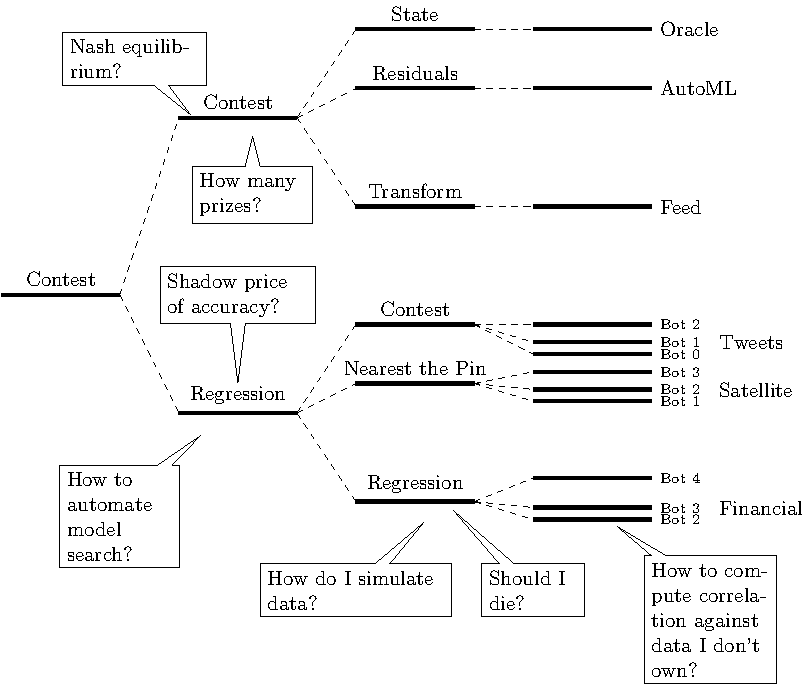
\includegraphics[width=1\textwidth]{03-oracles/PredictionWeb_tikz_oracle_graph.pdf}}
\else 
\fi 
\caption{Part of a microprediction web. An oracle answers prediction questions by fanning them out to micromanagers in real time, assessing longitudinal performance, and preparing an ensemble response. Algorithms can do the same, leading to a supply chain. Some managerial issues are suggested by questions, and discussed in later chapters.}
\label{fig:contest_of_contests}
\end{figure}


This realization is the moment of inception of the microprediction web.  

Because we cannot know the best way to combine models, and we cannot know the best way to manage in automated fashion a collection of models, we are drawn to something like figure \ref{fig:contest_of_contests} which is intended to represent a tower of micromanagers all trying to out-predict someone and, to better their chances, enlisting the expertise of other micromanagers who have access to additional techniques and data. 

If the top-level oracle is reactive (operates like a function responding to your prodding) then the more time given to respond to the question, and the lower the overhead for running a micromanager (i.e. fanout, management, etc) the deeper the calculation tree. The more micromanagers are involved, the greater the opportunity for specialization - not to mention broad data search.  

This diagram is intended to also convey some of the thorny questions that arise for micromanagers trying to survive in this game. 

The oracle property is evidently not a quality of a single micromanager. Rather, it emerges over time when a complex wiring of interrelated micromanagers is driven by greed. 

If we now suppose there are many users of many pseudo-oracles, and a rich variety of micromanagers tapping into multiple data sources, we have the beginnings of what we might call a microprediction web. 
\begin{quote}{Microprediction web definition}
A web-scale collection of radically low-cost self-organizing supply chains for microprediction, used almost universally to meet real-time operational needs.  
\end{quote}
(This definition implies reward-based decision-making by self-interested micromanagers, who are the economic agents.) An abbreviated plausibility argument that might lead one to speculate on this future possibility runs as follows.
\begin{quote}{Prediction web existence proof}
There is no definitive solution to the problem of automatically micromanaging algorithms that perform cost-aware repeated prediction, in order to achieve cost-aware repeated prediction ... and the rest follows.  
\end{quote}
But there must be something wrong with this proof, given the lack of existence of a microprediction web used universally across all industries! I posit:
\begin{enumerate}
    \item An inadequate supply of rewarded microprediction tasks. 
    \item Trade frictions
\end{enumerate}
My hope is that advertising the possibility of a prediction web might help with the first issue. Let's turn again to the second. 
\section{Overhead}





It is fair to say that our pseudo-oracle {\em encourages} a jumbled collection of nested and recurrent calls to micromanagers, including other pseudo-oracles (that precedes some eventual higher level recombination - and thereby an answer returned to the user). In conjunction with chapter \ref{chapter:economics}, this line of reasoning hopes to suggest that competitive tension is {\em necessary}.

Is it sufficient? One might cautiously say yes, the oracle definition appears to be met. For if it was easy to beat the output of this collective calculation, say with some new variety of neural network, then it should be relatively easy to endow said challenger with sufficient navigation ability (and economic common sense) that it finds its way across the network and addresses the problem. 

I mean, it would be if the network existed. Darn it. 

If we wish to understand why this dream is not already a reality, maybe it doesn't help to play with definitions. It perhaps pays to reiterate the critical assumption, however, or restate it thus:
\begin{quote}{The vanishing management principle}
   The overhead of managerial responsibility is eventually negligible. 
\end{quote}
where ``managerial responsibility'' includes the aforementioned challenge for itinerant algorithms. 

More colloquially put -- this is all bunk if nobody can be bothered running a contest, or can afford to. A time-series model might contain just a few lines of code, so in the absence of tooling, the additional work that allows the model to roam the world and find good uses might well swamp that effort. 

Our argument assumes that it is easy for anyone to also create imaginative variations on the general theme of a contest, and this would seem to be a non-trivial engineering problem. Can we really endow most of the world's data scientists with the ability to create micromanagers? 

It seems that everything will grind to a halt unless, to rephrase this ``overhead'' issue once more: 
\begin{quote}{Ratio test}
Micromanaging cost is small compared to the work that goes into designing self-contained algorithms. 
\end{quote}
Certainly we don't expect to see the microprediction web emerge on a platform that charges six figure sums to run a one-off contest. We {\em might} not see it if the rewarding is broken down into millions of individual proof-of-work transactions either, although all options should be explored. We won't pass the ratio test without supplying people with software. 

It is easy to fail the ``ratio test''. I do so constantly. For instance my attempt at a meta-time-series model mentioned previously doesn't pass muster. Nor does a group of people writing automated machine learning software. In these examples it is relatively expensive to tap into external sources of intelligence. (A human needs to write some code and send a pull request, typically). It feels too much like correspondence chess.  

As I sometimes refer to the buyer of microprediction as the parent and the suppliers (contestants) as children, I'd be tempted to call this test ``inexpensive parenting'' - if that wasn't such a dreadful oxymoron. For some applications, passing the ratio test may require tricks for dealing with volumetrics, migration of algorithms from child to parent, and other ideas. 

It is rarely obvious how best to engineer systems that will be improved by other people over time. It is even harder to pass the oracle test. We are demanding ongoing open competition, and at the same time we are suggesting that this should be easy to arrange. 

That idea is not entirely foreign. It is programmer lore that units tests are free, because they eventually save more time than they take to write (usually someone else's). But the engineering ambition, expressed in the ratio test, is that a rather more far-reaching test can also be close to free, even if that test might conceivably involve the whole world. 

For it is the whole world that might eventually solicit and combine predictions, data, features, hints or algorithms relevant to the problem at hand. Anyone should be able to engineer systems that are {\em automatically improved by other people and algorithms over time without their asking permission}. 

They should be able to do this without incurring any kind of high cost - be that code complexity, data expense, time on the calendar, or computational burden. If we can supply this ability to as many people as possible, by means of open source software and other conveniences, then maybe we'll get our microprediction web. 

\section{Example}

Confident in the march of technology, let's make our pseudo-oracle more concrete. This example is intended to illustrate that an ``edge'' micromanager (aspiring oracle, or pseudo-oracle) that faces application doesn't need to be perfect. 

\subsection{When Will the School Bus Arrive?}

What a fortunate life you live. Every day a yellow school bus pulls up to the top of your driveway and delivers your offspring. Your only task is to rush out -- typically in the middle of a meeting -- and meet them. 

The application we have in mind is purely passive. You do not do anything, beyond wearing your watch. However your watch will provide you with a two minute warning. Your driveway is rather long, we shall assume. 

Perhaps -- and now we're getting fancy -- you might input some indication of your cost function: how annoyed the school bus driver will be if you consistently leave them waiting. 

The application must be hungry for predictive intelligence. It will face competition from other applications like it. In the absence of a prediction web, the development of a state-of-the-art predictive model might chew up months. That model would be constantly revised. Data scientists might struggle with cleaning, extracting and use of data effectively - data drawn from a wide variety of sources with different formats.  

In order to remain popular in the eventually competitive bus-arrival genre {\em forever}, the application {\em eventually} needs to know all sorts of things. It needs data scraped from local sources. The bus is early when there is no band practice, late during certain special events, and later yet when Mrs Meldrum, your neighbor down the street, is asleep in her house (the driver has had to wake her once or twice -- her absence from social media is a status clue).   

The application logic, as distinct from the prediction logic, is pretty trivial. Your watch notices two events. The first event is your arrival near the top of your driveway. The second is your walking away. Typically the second event occurs several minutes after the first - or at least it used to before the invention of the prediction web. 

But now life is better because your watch can ping our pseudo-oracle, multiple times as needed, and receive good updated predictions of the estimated time of arrival. We imagine this is a cloud web service in this particular example (it wakes when a question arrives, does something, responds to you, and then goes back to sleep). 

The second event, your walking away from your letterbox, triggers a different type of message from your watch to the aspiring oracle. It sends an approximate ground truth, and while not absolutely necessary in every application, this certainly simplifies things.   

The running cost of this edge micromanager is measured in hundredths of a cent per month. Can it deliver that much value to you? We are about to find out because today, your watch held back on buzzing you for two minutes longer than usual. That's two whole minutes of sunshine you won't get in your over-optimized life.  

Still, it did give you time to finish that email, before walking out to meet your children. 

\subsection{Oracle implementation}

What does the pseudo-oracle do? As suggested by our reasoning, the oracle is a relay station that allows external people and algorithms to prove that they can predict the arrival time accurately. Put another way, it serves as an ongoing, real-time contest, as suggested by figure \ref{fig:bus}, and in this example it will do very little else. 

At the moment the oracle receives your question (``When will the bus arrive?''), it relays the question to a subset of the algorithms that have registered their interest. It will use its children to predict where yours are.

The watch app has conveyed, as part of the question, that it expects an answer within five seconds, so the oracle knows it had better establish a deadline for responses from children. That will allow it time to combine the results, and relay them to the watch. 


The oracle, or aspiring oracle we must remind ourselves, will also help initiate a relationship with other algorithms. We shall suppose it is implemented entirely reactively.


That is to say that the micromanaging pseudo-oracle answers the question ``when's the bus coming?'' but it also answers other types of questions that help other algorithms decide if they want to participate. For instance, the oracle might respond to questions like ``What's the prizemoney?'' with ``Not much, suck it up'' (or a more helpful numerical answer, maybe).   


\begin{figure}
\hspace{30mm}
\iftikz 
\makebox[0.2\textwidth][c]{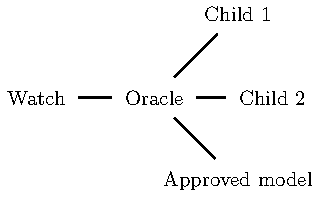
\includegraphics[width=0.45\textwidth]{03-oracles/PredictionWeb_tikz_oracle_contests.pdf}}
\else 
\fi 
\hspace{30mm}
\caption{A pseudo-oracle serves as a real-time contest between child 1, child 2 and others not shown. Both supply predictions of when a school bus will arrive. An approved model is used to bound perceived model risk.}
\label{fig:bus}
\end{figure}

Thus far, we've followed the previous script, but now we get into a small detail, because one of the children, called the ``approved model'' in figure \ref{fig:bus} is deemed special. 

A relatively simple, well-understood model for bus arrivals is used by the oracle to generate lower and upper bounds. This model assumes that the best estimate for the arrival time of the bus is an average of the last ten arrival times. It's not a great model, but regulators can understand it instantly, and it doesn't take long to document.   

\subsection{A modified median filter}

Upon receiving answers from the children the oracle must combine them and form a response for the watch. The first child's recency-weighted score is suggestively denoted $V_1$, the second $V_2$ and so forth. The oracle ranks the children by their (inaccuracy) scores from lowest to highest. The oracle then returns the median of the answers to the current question provided by the five children with lowest scores.

The exception is when that median differs from the approved model's answer by more than three minutes, whereupon the oracle adjusts the estimate closer to the approved model's answer until this is no longer the case. Thus every answer provided by the oracle is within three minutes of the approved model (for better or worse).  

A few minutes later the oracle receives the truth message. The bus actually arrived at 3.27pm. The first child predicted 3:28:10. The error in the estimate given by the first child is $70$ seconds. The squared error is $4900$. The aspiring oracle updates the child's score
$$
                \overbrace{V_1(new)}^{updated\ performance} = 0.99*\overbrace{V_1(old)}^{previous} + \underbrace{0.01}_{speed}*\overbrace{4900}^{score}
$$
and does the same for all children. In the event that a child fails to respond, or provides a badly formatted answer, it is put in the dog-house (just as you will be if you are consistently late). The child's score is reset:
$$
              \overbrace{V_1(new)}^{updated} = \underbrace{360000}_{reset\ inaccuracy}
$$
This amounts to a presumed standard error of ten minutes, which we assume is pretty poor.   

\subsection{Payouts}

I assume that periodically the oracle pays out accumulated prizes (received from the watch application) to children, according to their accuracy measured over some epoch (say a month). The most accurate model receives {\em half the total reward}. Less accurate contributors receive smaller prizes of $\frac{1}{4}$, $\frac{1}{8}$, $\frac{1}{16}$, $\frac{1}{16}$, based on both the accuracy and originality of their contribution. 

A simple way to define originality is by establishing an epoch-based priority scheme modeled after the patent system. Contributions are disqualified if they are consistently close to a contribution with greater vintage.  



\section{Analysis}

This completes the description of a very elementary attempt at an oracle. It may seem unlikely to meet our definition, but let's fast-forward several years. Perhaps by this time the arrival estimates are extremely accurate because everyone in your neighbourhood is using it, thereby generating more data and rewards. 

Perhaps by this time the small rewards have prompted someone to put a tracking device on the bus itself, thereby driving the prediction error to essentially zero. There is no such thing as cheating, in this particular contest. 

\subsection{Accomplishments}

The supply chain we have encouraged:
\begin{enumerate}
    \item permits granular contributions,
    \item and thus specialization, 
    \item and also cross subsidy (sharing of data and features),
    \item and possibly new data creation,
    \item with zero {\em mandated} human management or the inevitable overhead. 
\end{enumerate}
There are some possible downsides too, beginning with fear of opaque and changing model processes.  

\subsection{Model risk}

The beauty of the microprediction domain is that sometimes the so-called model risk is bounded. 

We merely observe that the oracle's predictions are ``explainable within three minutes'' and with that, the materiality of the model risk has been capped.

Bounding model risk isn't the same as bounding risk, it merely establishes that the risk is no worse, materially, than it is with any other solution that is considered to have acceptable model risk. (Please don't complain. Some if not most model risk policies are ridiculous due to the Stone-Weierstrass theorem, which can be translated to state that models with allegedly comprehensible risk are dense in the space of all models. What logic would you have me build on top of that quicksand?)

The use of the approved model isn't ``free'' -- by the way. If the bus can't start one day, and several models with superior data can discern this, too bad for you. The circuit-breaker will prevent you from being alerted to the full extent of the delay and therefore you may wait quite a while - albeit three minutes less than if you had relied only on an approved model.  

So by various metrics, there is a cost to using the approved model. However, on an amortized basis this cost is much smaller than other possible costs that might be imposed upon us - such as documenting, re-documenting, and re-documenting the operation of all models that contribute as they constantly improve. 

\subsection{Resistance to manipulation}

The aspiring oracle is designed with simplicity and robustness in mind. 

That's not to suggest we shouldn't be wary. A denial attack occurs when a participant clones the same entry many times (with a tiny amount of noise pollution). We will assume that this is defeated by the priority defence -- although in practice there are other defenses too. 


A Sybil attack, as we might term it, occurs when a nefarious source of intelligence creates three highly accurate prediction algorithms that are quite different yet outperform all others in the contest (the adversary may likely invest more effort than is warranted by the small rewards, in order to pull this off). Over the course of several months these entrants achieve the lowest error, thus taking control of the median. 

Then, one day, they conspire to return a bogus answer with the intent of deceiving you. The attack may persist for some number of days until the self-inflicted performance penalty moves the deceiving algorithms down the leaderboard. 

This doesn't cause great harm. The existence of an approved model and the bound means that the estimate will still be within three minutes of a half-way plausible guess. Not a catastrophic malfunction, by any means.



\subsection{Reliability}

No algorithm supplying predictions can be a single point of failure - except the approved model which is too dumb to fail. By encouraging diversity we become less reliant on any one algorithm performing when needed. We can fall back to the approved model, if need be. (Needless to say, there are more sophisticated methods of encouraging diversity than the simple system used in this example.)

To receive {\em any} payment an algorithm must also be accurate in its own right. So, if the top supplier drops out, the degradation in quality should not be extreme. There is incentive for all algorithms, however original, to improve their accuracy and maintain a spot near the top. 
 
There's a failure mode involving repeated fallback to the approved model - but that's easily detected. The oracle could even use another oracle for more advanced anomaly detection. 

\subsection{Eventually hard to beat?}

Now for the real exam. 

I turn to the question of the eventual efficiency - which is touted as the main selling point of the oracle. We observe that there are many things that might be considered questionable about the design. I have chosen a particular combination of model aggregation, and reward scheme, that is reasonably inoffensive, but not likely to be the best in any sense. 

I've noted in generality that there are many ways to reward and combine, and no way to know in advance what the best one will be. Even within the strictures of this narrow example, there are many choices to be made, such as the number of children ($5$) to include in the median, the speed parameter $(0.01)$, the reset inaccuracy score $(360,000)$, the exponent $(2)$ used to covert error into score, the count-back mechanism for prizes, and the payout fractions $\frac{1}{2},\frac{1}{4},\dots$. 

Furthermore, I make no claim that I am in the right {\em category of approach}. Should we use a precision-weighted estimate instead of the median, as suggested by the preceding discussion? 


And perhaps this micromanager simply isn't parenting enough. Our micromanager might lose out, in the long run, to a better parent that performs some critical pre-processing, or makes some auxiliary data easily available, or otherwise helps his or her children. 

And yet all these imperfections matter not, {\em up to a cost factor}, if there is no managerial overhead. That's because, as I've suggested in the description of the prediction web supply chains, it probably won't be individual models that are taking first prize but rather, a far superior generalized contest-like-construct. 

This ``better contest'' will be enriched, and can increase rewards paid to children. In turn it can attract its own better children, and so on. But the thing to notice is that this winning micromanager will receive half the prize-money. We are rewarding it, although perhaps not as much as we should. 

Yes, it would have been better to use it directly, instead of the unnecessary extra hop through our simple pseudo-oracle, but does that really matter all that much?  Let's look at this another way. In the long run, our unsophisticated oracle is {\em within a cost factor of two} of meeting the definition of an oracle!  

Lowering the cost of ``running a contest'' to zero begins to address the otherwise insurmountable problem of searching the world's data and models, in part by initiating a quest for better and better micromangers. An accuracy factor of two would be a concern. But given our working hypothesis that the current price of bespoke artificial intelligence is many orders of magnitude higher than it needs to be, a cost factor of two is not. 



\begin{figure}[htp]
\centering
\iftikz 
\makebox[0.38\textwidth][c]{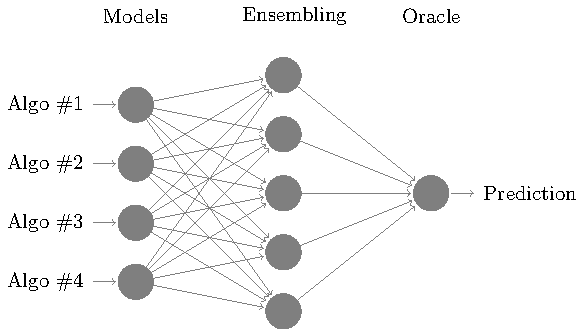
\includegraphics[width=1\textwidth]{03-oracles/PredictionWeb_tikz_oracle_contest_of_contests.pdf}}
\else 
\fi 
\caption{A contest between generalized contest mechanisms. A hypothetically superior method of sourcing and ensembling microprediction (generalized contest-like or market arrangements) can win half the prizemoney on offer. Thus a simple attempt at an oracle as we have described is within a cost factor of two of being as good as it might be.}
\label{fig_m_3}
\end{figure}

\subsection{What's missing?}

I use this bus stop oracle example to preempt and abstract objection to the use of microprediction oracles. 

A common critique is that powerful organizing principles have been eschewed in favour of a mechanical reward-based scheme that might not be best placed to bring domain knowledge to the problem, or otherwise tap generalized human intelligence. 

Notice that the oracle seems not to entertain norms, governance, culture, rules or other devices for binding people and machines together in productive fashion. It seems also to omit people from direct management, seemingly downplaying their ability to orchestrate quantitative work.  

In our setup, it certainly isn't a given that humans will get the opportunity to argue for hours in front of a whiteboard to determine which model goes into production. Nor will non-mathematical people get to provide meta-mathematical advice, or product flow diagrams, or otherwise engage in activities deemed useful in some circles. 

An overview of organizing principles is provided by Thomas Malone, who introduced the term {\em supermind} to refer to, and discussed strengths of, the combined activities of groups of people and machines.\endnote{ \cite{Malone2018HowWork}} 

In search of superminds to compete with our perfunctory streaming contest, we scan the history of human civilization and find, among other things, nuanced examples of competing political systems - with all their rules, procedures, checks and balances. More broadly, millions of different kinds of groups of people somehow have got along (I'd cautiously suggest that no two book clubs follow precisely the same set of protocols) many with specific engineering objectives in mind. 

I'd agree that the rich diversity of ways in which humans have coalesced around projects, each with different expectations placed on contributors,  makes for an uncomfortable juxtaposition with the rudimentary ``micro-greed'' presented. 


Yet while it is trivial, the pseudo-oracle as described nonetheless {\em does} organize humans and machines. Moreover, and more critically to the argument, it is a methodology for {\em assessment of other organizing principles} - the real beauty of this particular micromanager and many like it. 

So in fact we will get to see if obscure social norms and daily stand-up routines binding the People's Front of Judea are precisely what is needed to organize collective quantitative work. Or maybe the Judean People's Front, with closer allegiance to proletarian futarky, will do better. One of these groups might sooner or later be able to beat all others on an accuracy and cost basis. 

I was honest at the outset of this book that I was intent on reducing the problem to one with a solution. We can only collapse this huge discussion because the domain is microprediction: frequently repeated prediction where assessment of performance by mechanical means is warranted. 

(I may have pushed the boundaries using daily questions in this example, but if enough of us use the app we'll get away with it sooner or later.) 

No, an oracle can't tell you if the Westminster system is better than a presidential democracy. It only delineates microprediction superminds, and as noted you might pay for that.  

Yet in this line of argument I don't mean to surrender the contest between contests to human managers so easily - and nor do they seem likely to win in many cases.   
For it is worthy of mention, although not essential to the logic, that in many cases the human centered efforts will be undercut by more efficient use of generalized intelligence. A micromanager can chronicle its exploits and experimentation, and ask for help occasionally. It can generate questions a human can answer is a very short amount of time, thereby including domain knowledge. 

For example a micromanager can pay one cent to glean an opinion from a human as to the plausibility of local weather impacting bus arrival. If it spends three cents, it will probably come away with a reasonable degree of confidence in the answer. That's not hard to accomplish using Amazon Turk, named for the fake chess playing machine of the 18th Century, or other crowd-sourcing software.  

Jeff Bezos referred to Amazon Turk as artificial artificial intelligence. A dash here and there goes a long way.  




\section{Summary}


Gordon Gekko said that greed is good - not perfect. At a small cost it is good enough, in the microprediction domain, to locate a superior organizing principle (should one exist). 

I've described a hypothetical prediction web as a vast collection of intertwined, miniature supply chains for repeated short term prediction, in which micromanagers play the role of value adding firms. 


I've suggested that one day, it might be difficult to avoid making use of this utility. Applications will be able to access this power using functions or API's, termed oracles, that can aspire to be eventually hard to beat based on the collective properties of the micro-economy. 


While simple and seemingly insignificant, the bus arrival application is an interesting little wedge. It illustrates the rudimentary notion of a minimalist microprediction micromanager that asks others to do its bidding. Yet this toy sooner or later provides the most accurate microprediction that {\em twice your money} can buy. It's almost an oracle! 

And through this rendering we arrive at a seemingly strange conclusion: that the real problem we wish to solve is only incidentally related to machine learning techniques per se. Making better algorithms is a noble goal, but it isn't the blocker when it comes to making microprediction, and thus what passes for AI, better faster and cheaper for everyone.  

Instead, the actual challenge is the task of driving down the relative cost of automated management of contributions, which might take the form of a real-time machine learning contest, or generalizations of that concept that we will discuss in more detail in chapter \ref{chapter:mental}. 

However before investing effort in further speculation about the interior of the microprediction web, and the micromanagers that inhabit it, I will turn to a slightly broader justification of this line of thinking. 


   





















